% This is "sig-alternate.tex" V2.1 April 2013
% This file should be compiled with V2.8 of "sig-alternate.cls" May 2012
%
% This example file demonstrates the use of the 'sig-alternate.cls'
% V2.8 LaTeX2e document class file. It is for those submitting
% articles to ACM Conference Proceedings WHO DO NOT WISH TO
% STRICTLY ADHERE TO THE SIGS (PUBS-BOARD-ENDORSED) STYLE.
% The 'sig-alternate.cls' file will produce a similar-looking,
% albeit, 'tighter' paper resulting in, invariably, fewer pages.
%
% ----------------------------------------------------------------------------------------------------------------
% This .tex file (and associated .cls V2.8) produces:
%       1) The Permission Statement
%       2) The Conference (location) Info information
%       3) The Copyright Line with ACM data
%       4) NO page numbers
%
% as against the acm_proc_article-sp.cls file which
% DOES NOT produce 1) thru' 3) above.
%
% Using 'sig-alternate.cls' you have control, however, from within
% the source .tex file, over both the CopyrightYear
% (defaulted to 200X) and the ACM Copyright Data
% (defaulted to X-XXXXX-XX-X/XX/XX).
% e.g.
% \CopyrightYear{2007} will cause 2007 to appear in the copyright line.
% \crdata{0-12345-67-8/90/12} will cause 0-12345-67-8/90/12 to appear in the copyright line.
%
% ---------------------------------------------------------------------------------------------------------------
% This .tex source is an example which *does* use
% the .bib file (from which the .bbl file % is produced).
% REMEMBER HOWEVER: After having produced the .bbl file,
% and prior to final submission, you *NEED* to 'insert'
% your .bbl file into your source .tex file so as to provide
% ONE 'self-contained' source file.
%
% ================= IF YOU HAVE QUESTIONS =======================
% Questions regarding the SIGS styles, SIGS policies and
% procedures, Conferences etc. should be sent to
% Adrienne Griscti (griscti@acm.org)
%
% Technical questions _only_ to
% Gerald Murray (murray@hq.acm.org)
% ===============================================================
%
% For tracking purposes - this is V2.0 - May 2012

\documentclass{sig-alternate}

%\usepackage[latin1]{inputenc} % Windows
\usepackage[utf8x]{inputenc} % Linux (unicode package needed)
% \usepackage[applemac]{inputenc} % Mac

\usepackage{balance}

\usepackage{graphicx}
\usepackage{caption}
\usepackage{subcaption}
\usepackage{hyperref}

\usepackage{listings}
\usepackage{xcolor}


\colorlet{punct}{red!60!black}
\definecolor{background}{HTML}{FEFEFE}
\definecolor{delim}{RGB}{20,105,176}
\colorlet{numb}{magenta!60!black}

\lstdefinelanguage{json}{
    basicstyle=\small\ttfamily,
    % numbers=left,
    % numberstyle=\scriptsize,
    % stepnumber=1,
    % numbersep=8pt,
    % showstringspaces=false,
    % breaklines=true,
    % frame=lines,
    backgroundcolor=\color{background},
    literate=
     *{0}{{{\color{numb}0}}}{1}
      {1}{{{\color{numb}1}}}{1}
      {2}{{{\color{numb}2}}}{1}
      {3}{{{\color{numb}3}}}{1}
      {4}{{{\color{numb}4}}}{1}
      {5}{{{\color{numb}5}}}{1}
      {6}{{{\color{numb}6}}}{1}
      {7}{{{\color{numb}7}}}{1}
      {8}{{{\color{numb}8}}}{1}
      {9}{{{\color{numb}9}}}{1}
      {:}{{{\color{punct}{:}}}}{1}
      {,}{{{\color{punct}{,}}}}{1}
      {\{}{{{\color{delim}{\{}}}}{1}
      {\}}{{{\color{delim}{\}}}}}{1}
      {[}{{{\color{delim}{[}}}}{1}
      {]}{{{\color{delim}{]}}}}{1},
}

\begin{document}

% Copyright
\setcopyright{acmcopyright}
%\setcopyright{acmlicensed}
%\setcopyright{rightsretained}
%\setcopyright{usgov}
%\setcopyright{usgovmixed}
%\setcopyright{cagov}
%\setcopyright{cagovmixed}


% DOI
\doi{10.475/123_4}

% ISBN
\isbn{123-4567-24-567/08/06}

%Conference
\conferenceinfo{DocEng2015}{Sep 8--11, 2015, Lausanne, Switzerland}

\acmPrice{\$15.00}

\title{HiJson: a cartographic document format for web modeling 
of interactive indoor mapping}


\numberofauthors{6}
\author{
\alignauthor
Marco Virgadamo\\
 \affaddr{Dipartimento di Ingegneria}\\
 \affaddr{Universit\`a Roma Tre}\\
 \affaddr{Rome, Italy}\\
 \email{virgadamo@dia.uniroma3.it}
\alignauthor
Marco Sportillo\\
 \affaddr{Dipartimento di Ingegneria}\\
 \affaddr{Universit\`a Roma Tre}\\
 \affaddr{Rome, Italy}\\
 \email{sportillo@dia.uniroma3.it}
\alignauthor 
Federico Spini\\
 \affaddr{Dipartimento di Ingegneria}\\
 \affaddr{Universit\`a Roma Tre}\\
 \affaddr{Rome, Italy}\\
 \email{spini@dia.uniroma3.it}
\and % use '\and' if you need 'another row' of author names
\alignauthor 
Alberto Paoluzzi\\
 \affaddr{Dip. di Matematica e Fisica}\\
 \affaddr{Universit\`a Roma Tre}\\
 \affaddr{Rome, Italy}\\
 \email{paoluzzi@dia.uniroma3.it}
\alignauthor 
Enrico Marino\\
 \affaddr{Dipartimento di Ingegneria}\\
 \affaddr{Universit\`a Roma Tre}\\
 \affaddr{Rome, Italy}\\
 \email{marino@dia.uniroma3.it}
\alignauthor 
Antonio Bottaro\\
 \affaddr{Sogei S.p.A.}\\
 \affaddr{Ricerca e Sviluppo}\\
 \affaddr{Rome, Italy}\\
 \email{abottaro@sogei.it}
}

\date{23 March 2015}
\maketitle
%\section{}
%\subsection{}


\begin{abstract}
This paper introduces HiJson\footnote{This work was partially supported by grant 2014/15 from Sogei S.p.A., the ICT company of the Italian Ministry of Economy and Finance.}, a novel indoor cartographic document format. A software framework is also presented, that relies on HiJson documents and is entirely based on web technologies. With respect to current cartographic formats, HiJson suggests four major enhancements: (a) exposes a hierarchical structure; (b) uses local metric coordinate systems; (c) may import external geometric models; (d) accepts semantic extensions. The semantic extensions supported by the HiJson framework architecture encapsulate the details about communication protocols, rendering style, and exchanged and displayed information, allowing the HiJson format to be extended with any sort of models of objects, sensors or behaviors.
\end{abstract}


\section{Introduction}

For environments with massive presence of sensor-equipped (or ``smart") objects, which realize the socalled IoT (Internet of Things), the interactive indoor mapping represents an ideal integrated interface for IoT monitoring systems. To be specific, it can be the container of indoor navigation systems, giving the user, to be routed across an indoor environment, the opportunity to interact with objects along the suggested paths. Furthermore, in conjunction with the advancements in the field of user indoor location, whose efforts are nowadays focused to realize an integration of positioning systems like GNSS (Global Navigation Satellite system), Wi-Fi, Bluetooth and LTE (Long Term Evolution), to support continuos outdoor/indoor navigation by means of integration of technologies, it represents the most natural interface to perform realtime access monitoring and multi-person tracking.

An interactive mapping platform allows the representation of the indoor environment of  both public or commercial places of vast dimensions, as for example airports, train stations, shopping malls, and also private buildings subject to strict access protocols, like warehouses, logistic centers, data centers, etc.
Despite of the growing attention regarding indoor cartography, efforts to specify open formats for indoor representation are few and partial, and certainly not intended to support the interactive indoor mapping, which is conversely the main purpose of this paper.

Research on the cartographic representation of indoor environments is extensive and heterogeneous with respect to the strategies applied~\cite{6418876}. Different information sources are used, and accuracy of the produced solution depends on the adopted approach. In some cases the information is obtained with automatic or semi-automatic processing of files that describe the architectural structure of a building, such as BIM (Building Information Modeling)~\cite{Eastman:2008:BHG:1796500} and/or IFC (Industry Foundation Classes) that describe a building project [4]. 
The actual ``de-facto" standard in terms of geospatial data representation is the GeoJSON format, which can be easily used for any type of geographical annotation. In some cases it has been slightly adapted to be used in indoor environments: it is the case of the IndoorJSON format.


\section{Our contribution}

The focus of this work is the definition of a novel format of cartographic documents along with the software ecosystem rooted on it. HiJson (Hierarchical Indoor JSON) is the name chosen for the new document format; with the accompanying software framework, aims to realize a mapping between the real indoor spaces and a virtual interactive web environment. A simple but effective algorithm to find indoor valid routes is also provided. 

\paragraph{Hierarchical structure}

The HiJson format allows for hierarchical description of indoor spaces, reflecting a container-contained relationship. This directly implies a neater representation then the plain linear structure adopted by GeoJSON, being a perfect analogy of objects contained (i.e. placed) into spaces.
Therefore, an organized arrangement of spaces is allowed by HiJson, via logical (or even physical) grouping: concepts like building wings, sections, storeys, departments, etc. can be directly introduced, in order to reflect into the document structure the actual logical or physical divisions, categories or relationships among the modelled spaces.
Furthermore, the container-contained relation enables a recurring use of local reference frames.

\paragraph{Metric local coordinate system}

Supported by the hierarchical underlying structure, the HiJson document format allows the use of local coordinate systems. Hence the shape of all elements can be conveniently modelled using local coordinates, and then placed in the right position with respect to the position of the parent (or container) element applying a rotation, followed by a translation transformation.
Another substantial advantage is represented by the adoption of a metric reference frame, consequently simplifying the compilation of the document, either manually generated or produced by software tools. Just remember that the GeoJSON coordinates are geographical, a pairs of (absolute) latitude and longitude angles, like the ones provided by GNSS systems. This kind of coordinates are certainly not particularly user friendly, when positioning a smart device or a furniture element within a specific building room.

\paragraph{Hyperlinked geometric models}

The HiJson document may further import external geometric models | either of the buildings themselves or the interior furniture or devices | that are topologically complete (in the sense of solid modeling [15]) and very compact. Such models, coming from a source outside the document, are acquired by hyperlinking JSON files that contain a Linear Algebraic Representation (LAR) of topology and geometry, to be expanded for visualization or interaction at any useful level of detail.
The LAR scheme~\cite{Dicarlo:2014:TNL:2543138.2543294} is characterised by a very large domain, including architecture, building and construction~\cite{paoluzziMS:2014}, 2D and 3D engineering meshes, non-manifold geometric and solid models and meshes, and high-resolution 3D images~\cite{cadanda:2015}. 
The expansion of a LAR model, to be considered as a general-purpose graphic primitive, may be executed on either the server or the supervisor client of the HiJson Web Toolkit architecture (see Section 6.2.1), or even on the Explorer client.

\paragraph{Semantic extensions}
Semantic extensions make the HiJson format extendible and customizable, that is able to adequately respond to any need of objects representation. To define a semantic extension means to allow the HiJson document to model an object previously not covered, or even to modify the behavior of a comprised one. Semantic extensions are to be defined both as HiJson format syntax and as HiJson Toolkit source code. In particular it is necessary to define respectively a new HiJson Element and a new HiJson Class.

\begin{figure*}[tbh]
 \centering
 ~
 \begin{subfigure}[b]{0.27\linewidth}
 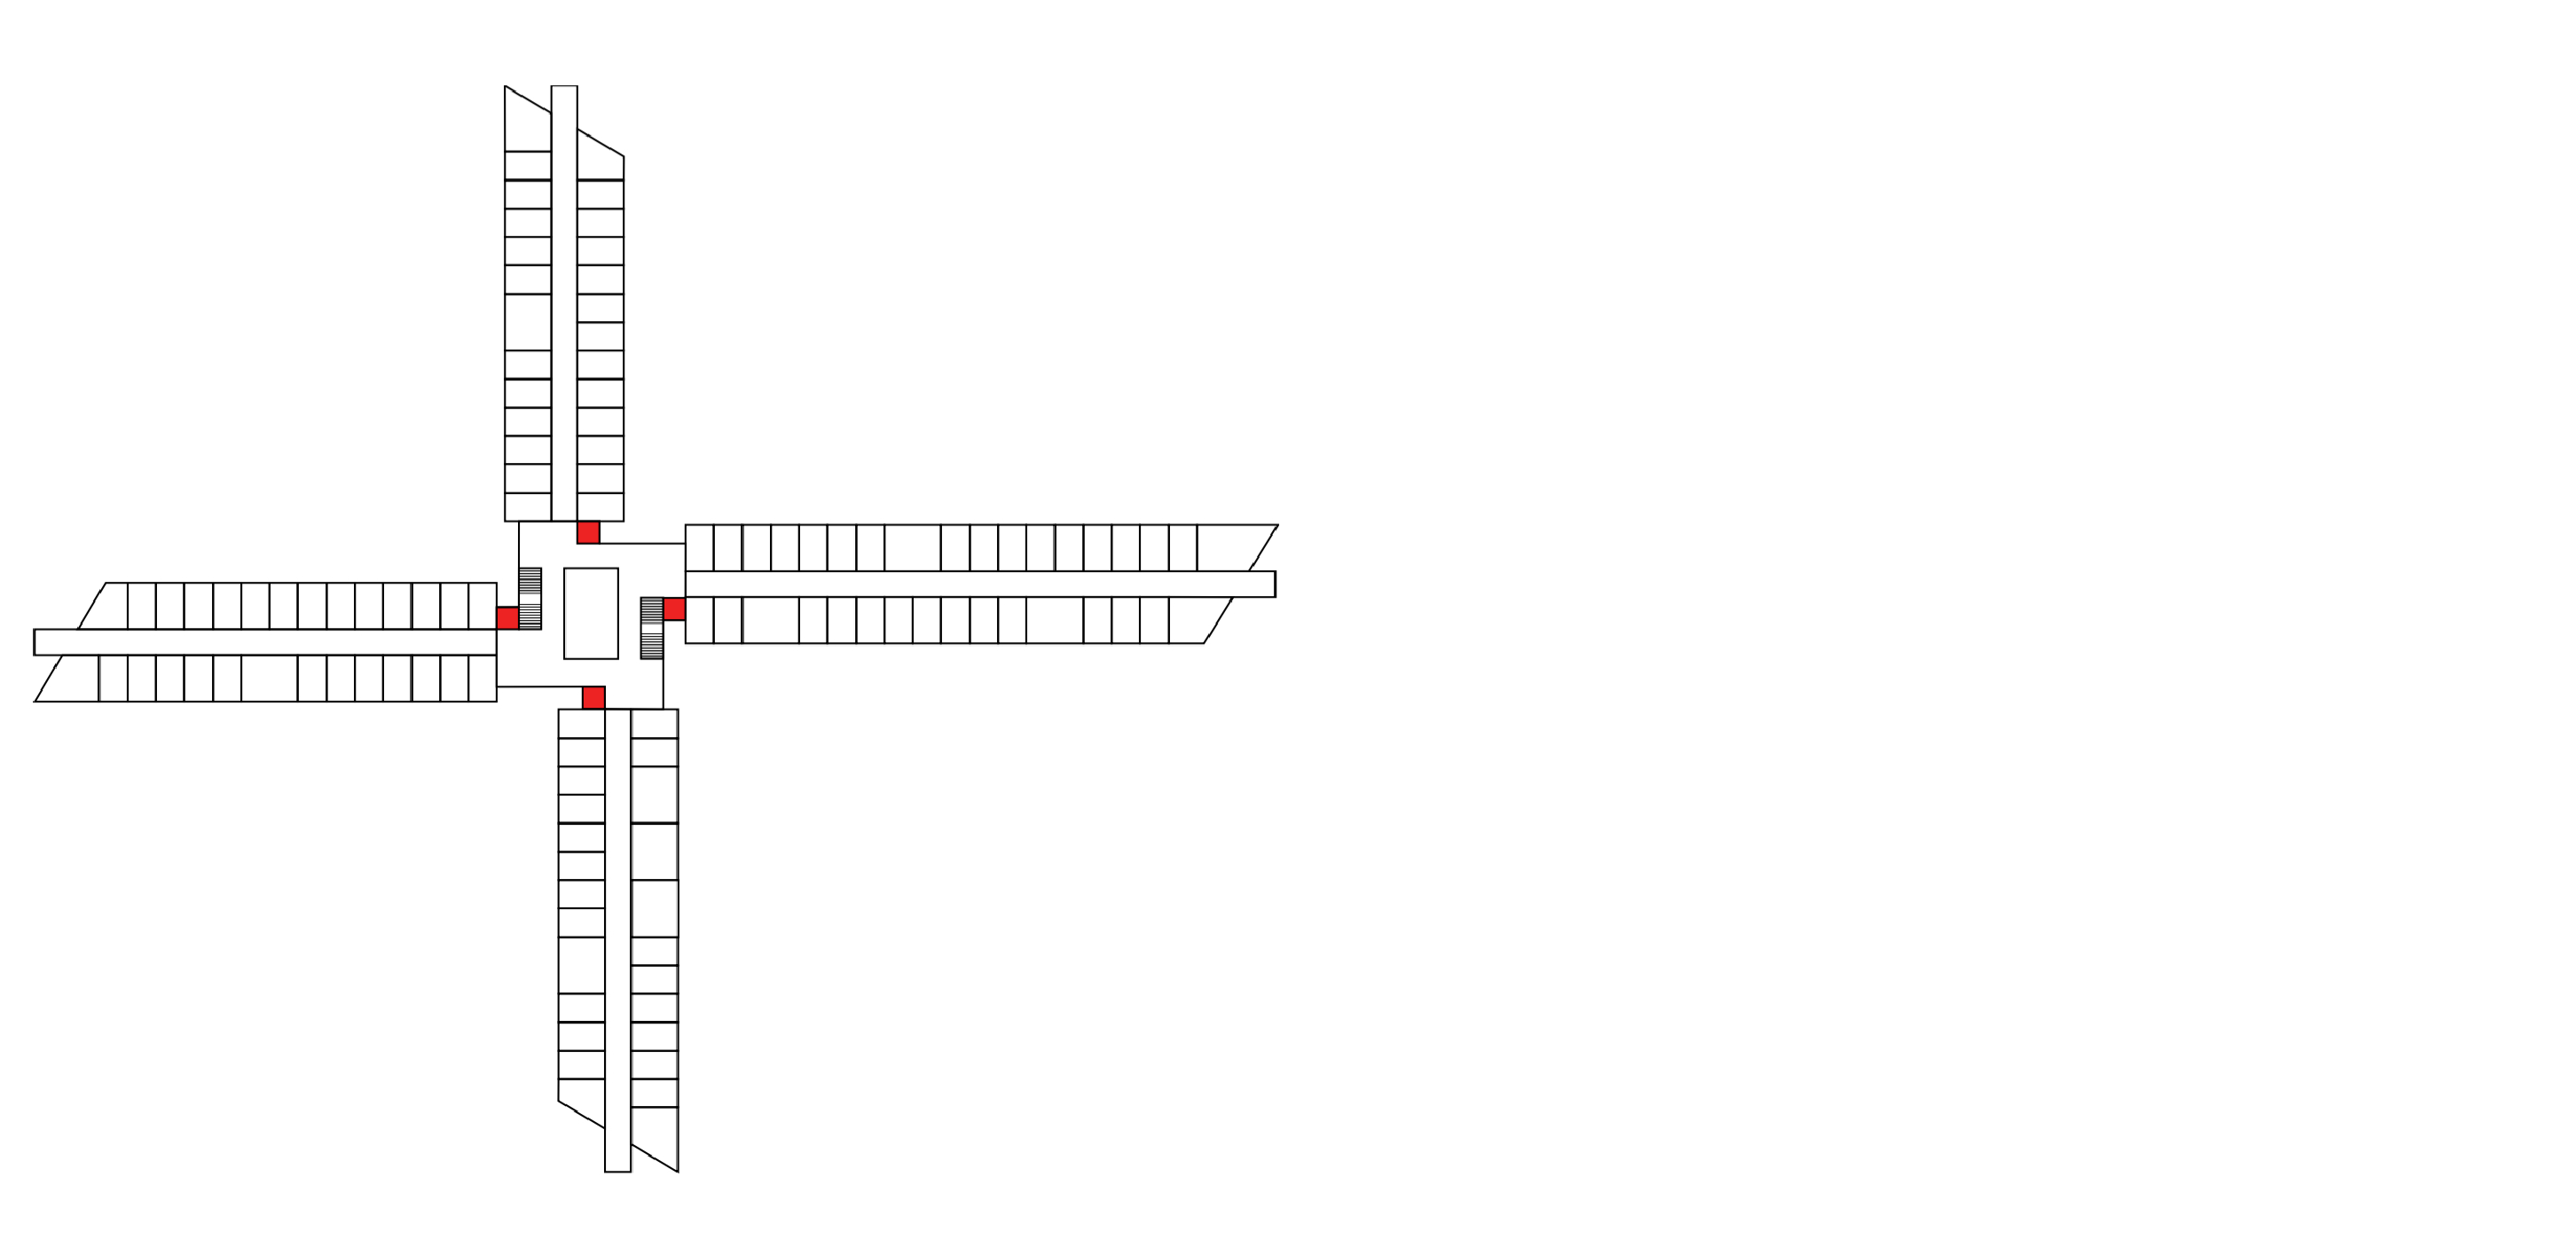
\includegraphics[width=\textwidth]{../images/sogei-a} 
 \end{subfigure}
\hfill
 \begin{subfigure}[b]{0.33\linewidth}
 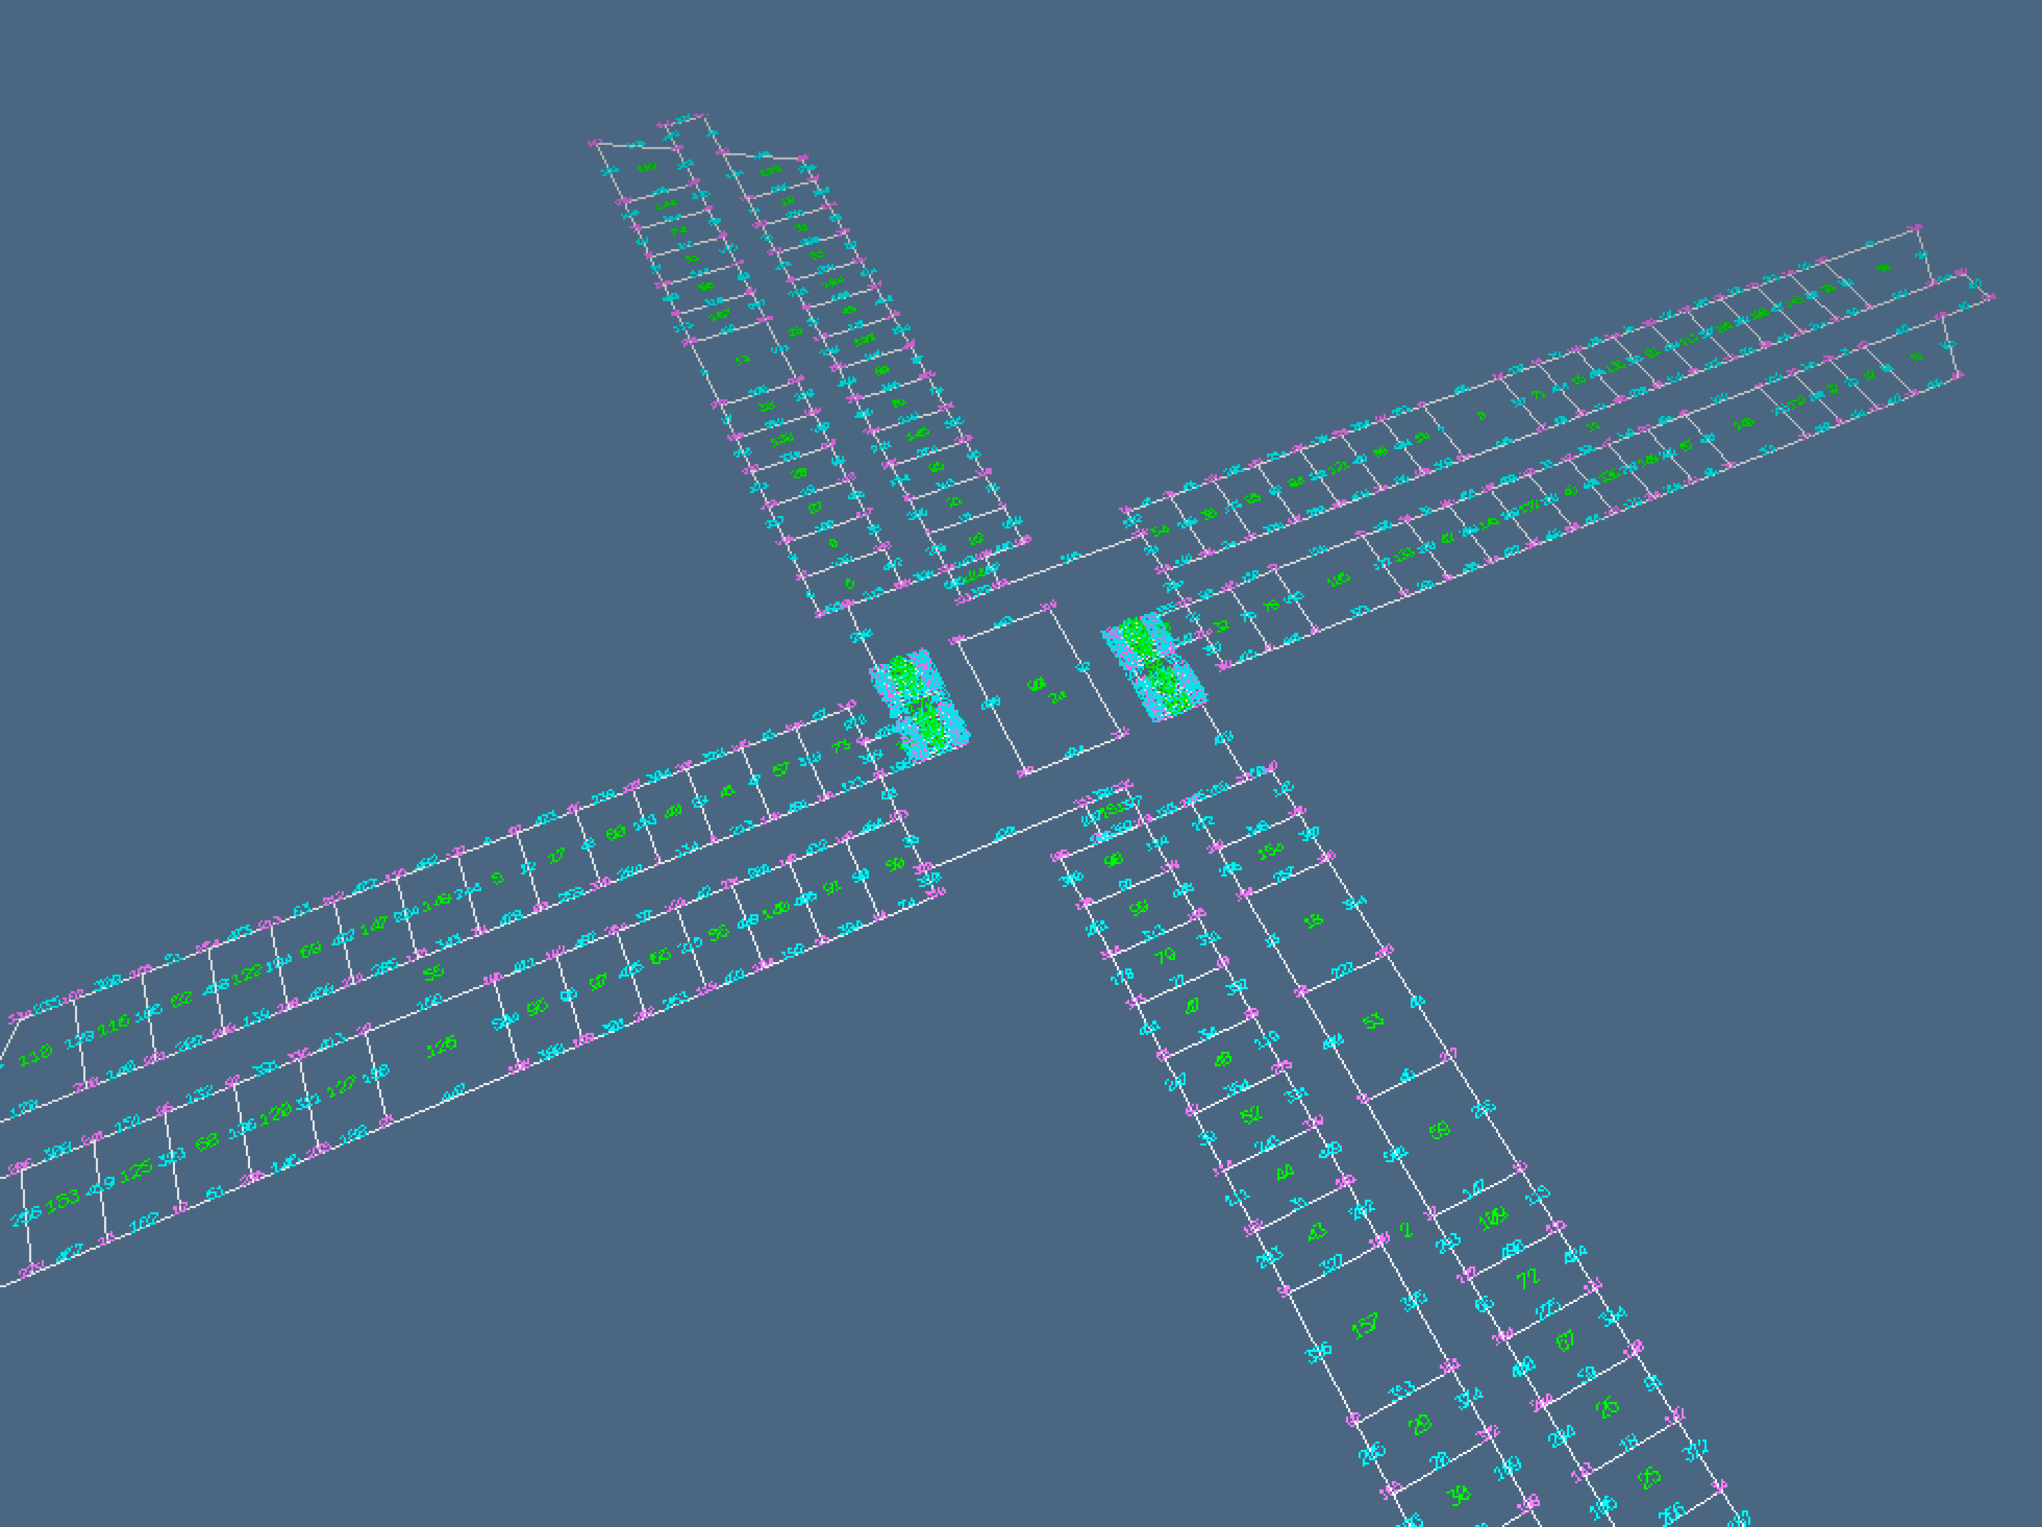
\includegraphics[width=\textwidth]{../images/building} 
 \end{subfigure}
\hfill
 \begin{subfigure}[b]{0.27\linewidth}
 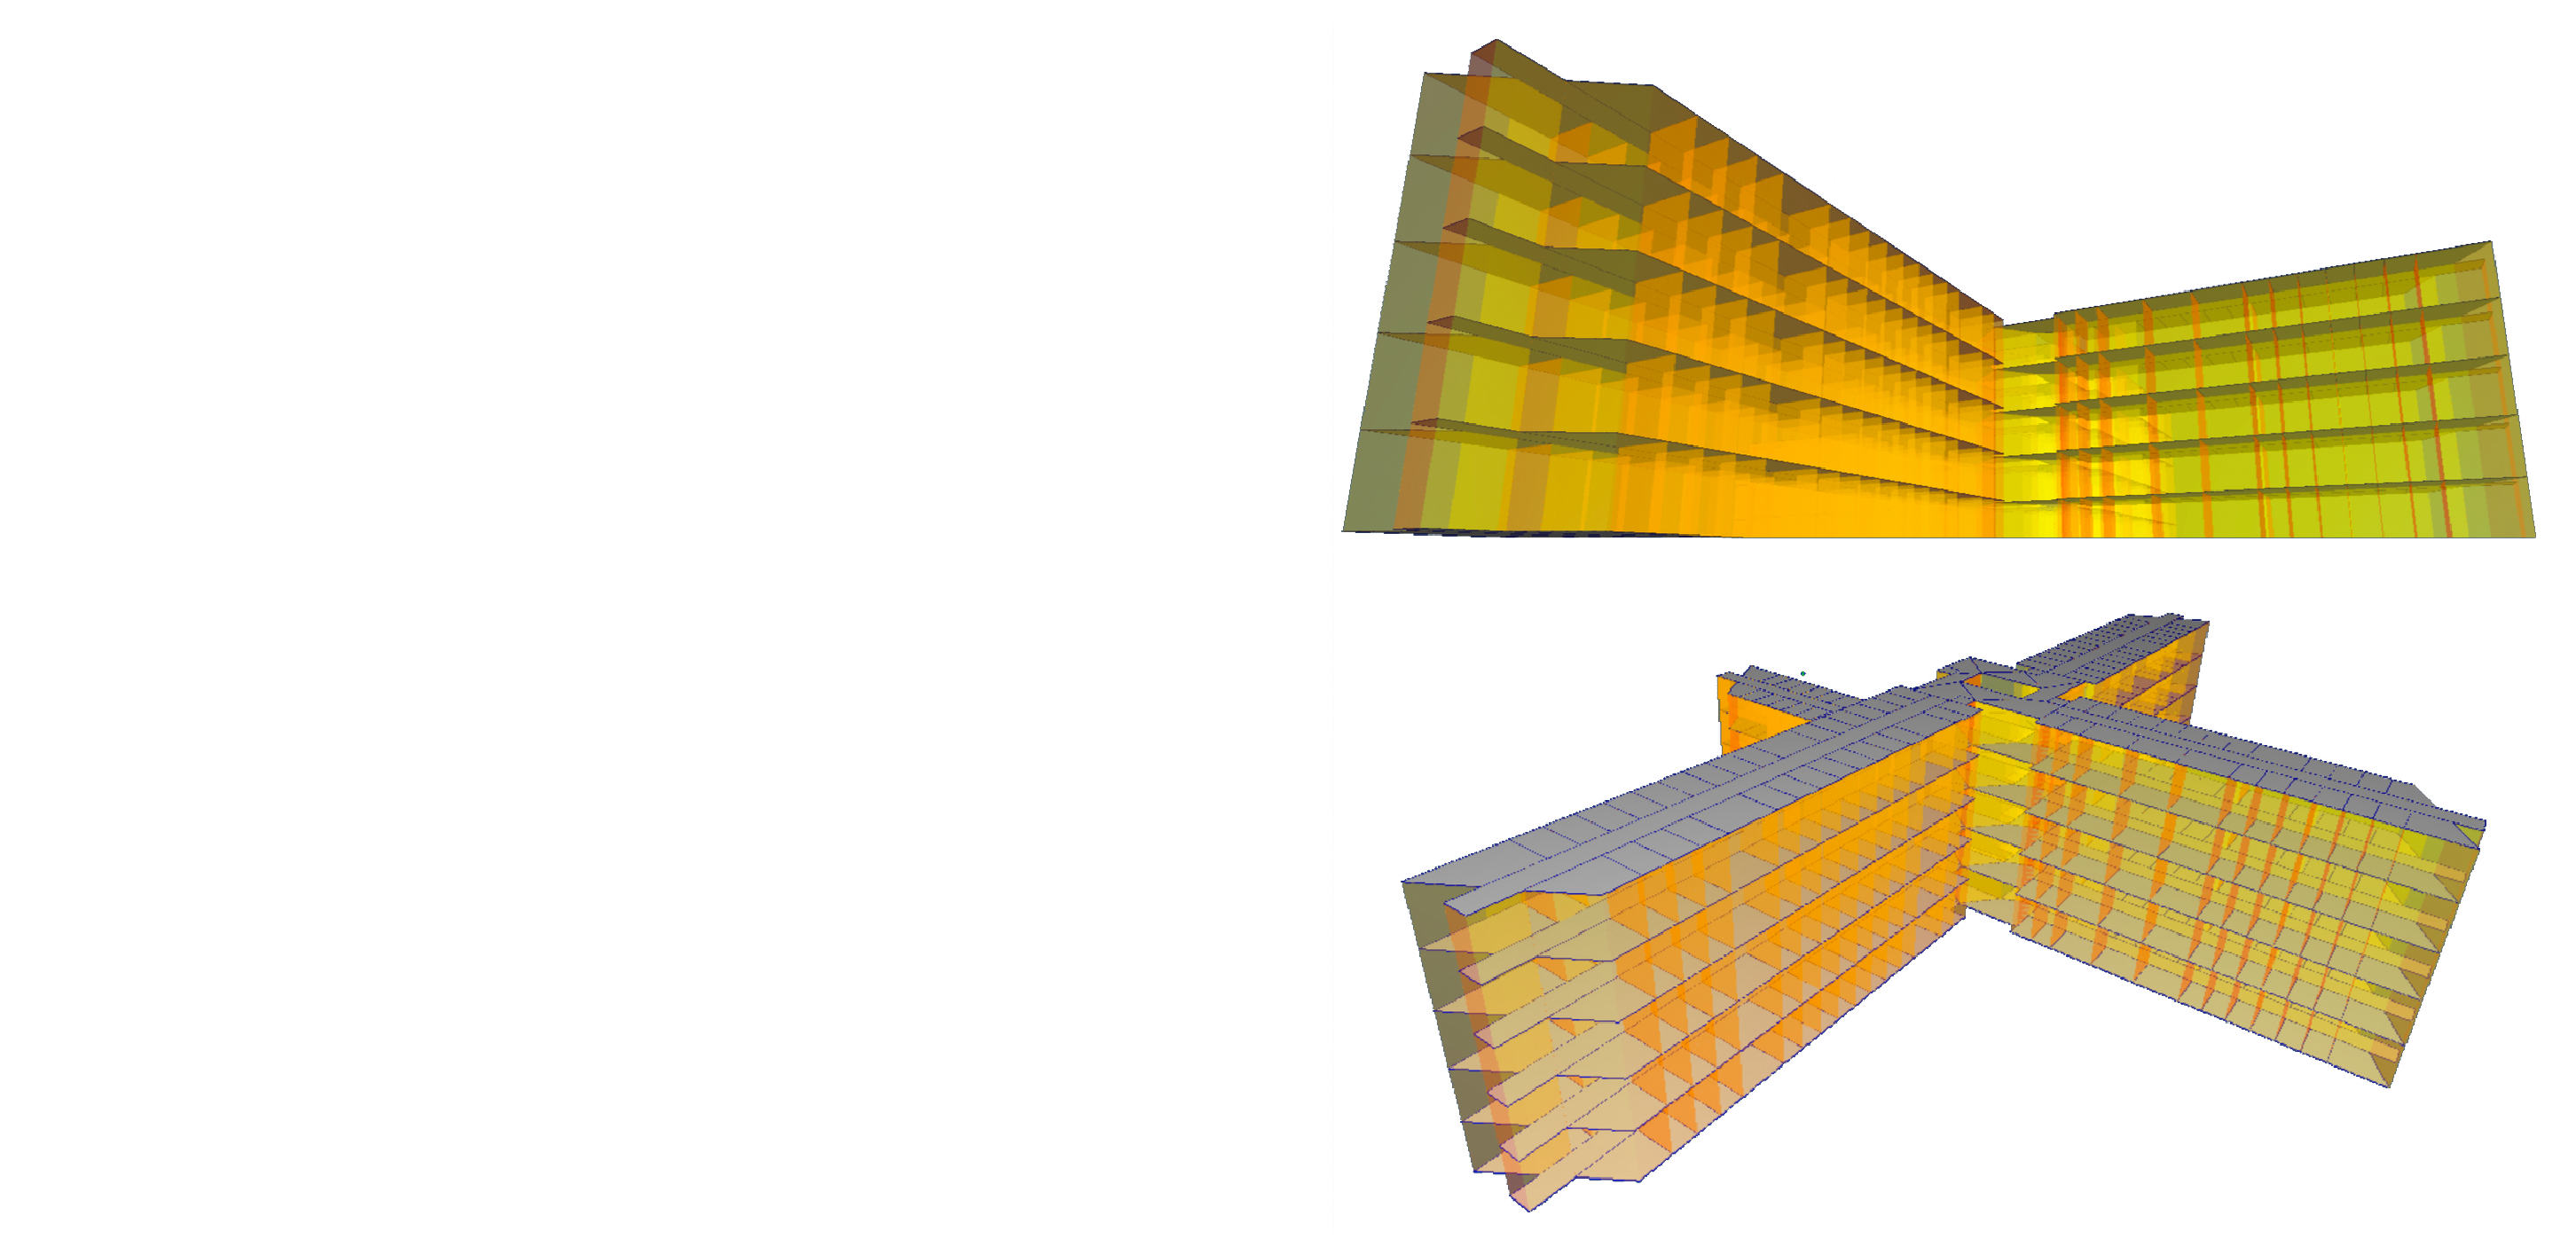
\includegraphics[width=\textwidth]{../images/sogei-b}
 \end{subfigure}
 \caption{Office building: 
 (a) the schematic plan---made of SVG primitives: lines, rects, polygons---possibly obtained via a client UI loading engineering design in background;
 (b) the automatically generated LAR cellular complex, transformed server-side into HiJson; 
 (c)~the mock-up for the automatically generated 3D HiJson.
 }
 \label{fig:sogei}
\end{figure*}


\begin{figure}[tbp]
 \centering
 \begin{subfigure}[b]{0.1\textwidth}
 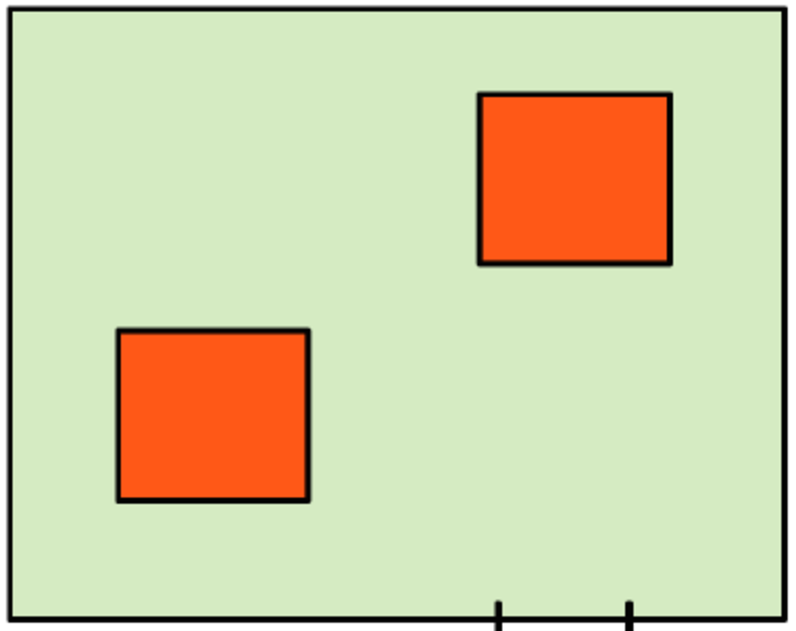
\includegraphics[width=\textwidth]{../images/graph-new-1}
 \end{subfigure}
 ~
 \begin{subfigure}[b]{0.1\textwidth}
 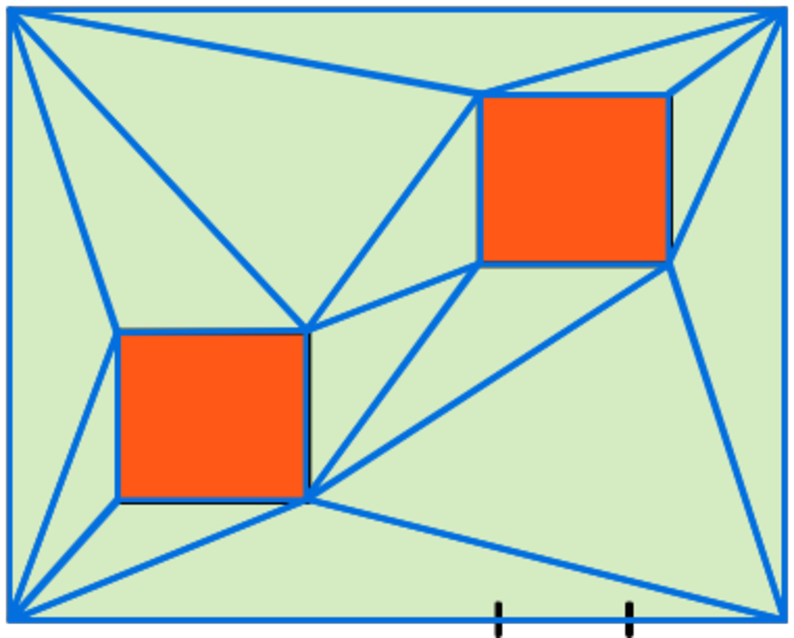
\includegraphics[width=\textwidth]{../images/graph-new-2}
 \end{subfigure}
 ~
 \begin{subfigure}[b]{0.1\textwidth}
 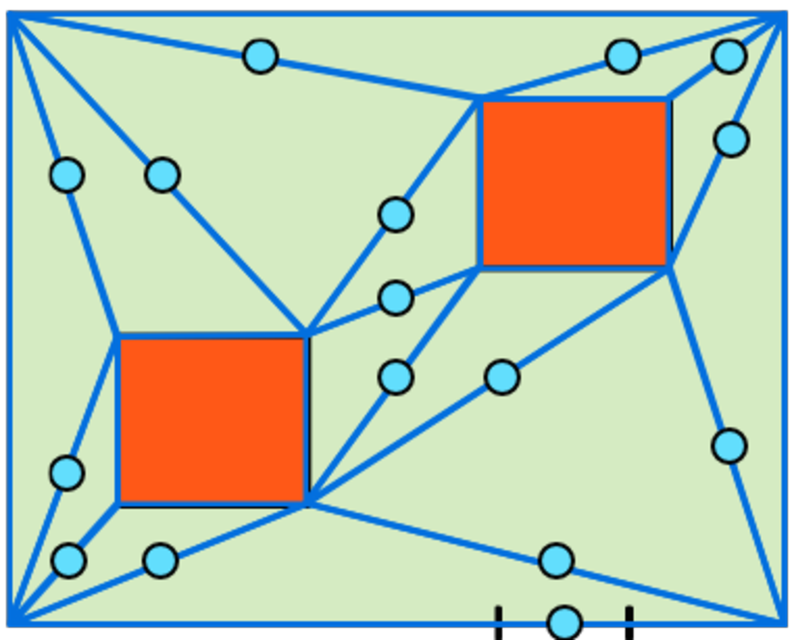
\includegraphics[width=\textwidth]{../images/graph-new-3}
 \end{subfigure}
 ~
 \begin{subfigure}[b]{0.1\textwidth}
 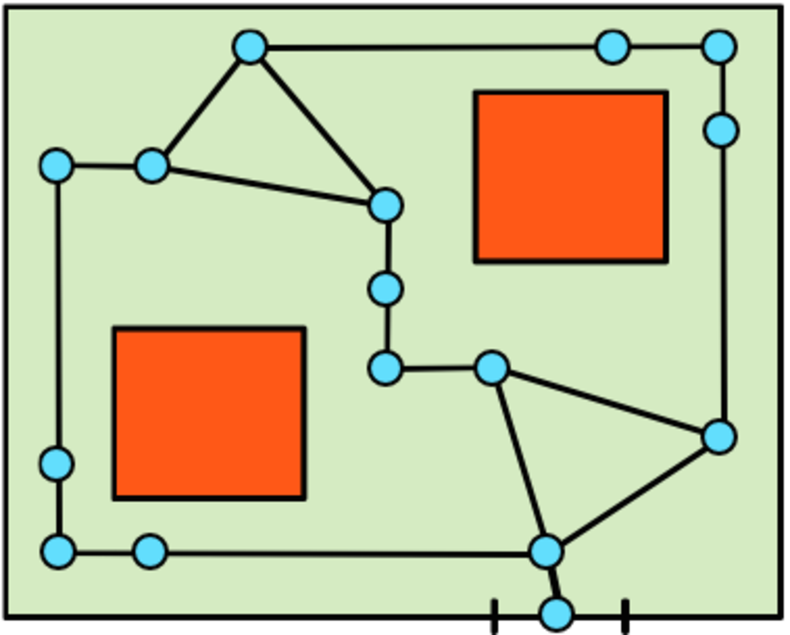
\includegraphics[width=\textwidth]{../images/graph-new-4}
 \end{subfigure}
 
 \caption{graph of paths generation: 
 (a) detection of obstacles and computation of walkable area; 
 (b) triangulation of walkable area; 
 (c) identification of graph nodes; 
 (d) junction of nodes.
 }
 \label{fig:graph-generation}
\end{figure}

\section{HiJson ecosystem}


\subsection{HiJson Document}

The HiJson document is composed by a configuration section, followed by one or more FeatureCollections, containing the actual data.


The configuration part includes parameters and settings needed for building representation in the form of a JSON Object. One of the core information in this section is defined by the correspondence between three points of the local coordinate system and three points of the real world, expressed in geographical coordinates. This is needed to ensure a seamlessly passage from local to geographical coordinate system and vice versa.

After the configuration section, the document includes a list of FeatureCollection. 
Each element of the list is given in the form of a GeoJSON FeatureCollection, that contains an arbitrary number of HiJson Elements. Each FeatureCollection imposes a logical relationship that can be used to group together related HiJson Elements. Since HiJson Elements adhere to the GeoJSON format, each FeatureCollection results compliant with GeoJSON syntax and then accepted by any GeoJSON validator. 

Dealing with indoor environments, there are essentially two classes of objects that is necessary to represent. They are (a) architectural elements, like a room, a corridor, a wall, etc. and (b) furnishings, intended in a broad sense, such as to contain both furniture, like a desk or a chair, and/or ``smart objects", like an IP-cam or a connected thermostat.

The hierarchical structure of the document gives visible form to the capability of HiJson Elements to have children elements. A unique ID is mandatory for every HiJson Element.
Three Geometry types can be used here: Point, LineString and Polygon. The choice of the Geometry type to be associated to a HiJson Element implicitly defines the category of the element: Point is used for furnishings, LineString for walls and doors, while Polygon may describe levels and rooms.
The Geometry coordinates are expressed in metres, by convention starting at the bottom-left corner of the element, whose position is used to set-up the origin of a local coordinate frame. 

\subsection{HiJson toolkit}

The HiJson Toolkit is a software module that implements common operations and transformations on HiJson documents. Written in JavaScript language, this software module has been built to be deployed in the web environment. It is modular and entirely isomorphic, i.e. can run on the server as well as on every client. Working in the web environment, the Toolkit benefits of the ``fertility" commonly concerning the software development in this field: for example, it takes advantage of libraries and frameworks such as React, ``the JavaScript library for building user interfaces" by Facebook, and as Three.js, the current de-facto standard to deal with WebGL technologies.

\paragraph{Processing pipeline} 
The HiJson processing pipeline implements the sequence of preliminary transformations that have to be applied to a HiJson document before any further operation. It is not strictly required to complete each stage of the pipeline: the exit stage depends on the specific use case.

The application of the transformation pipeline has a double aim. The first one consists in generating the graph of valid paths among all the interesting elements. The second objective is the generation of one GeoJSON document for each storey of the building described by the HiJson document. In this way a bidimensional layout can be provided for every level of the building, and visualized through any compliant GeoJSON viewer.

\begin{figure}[!htbp]
\centering
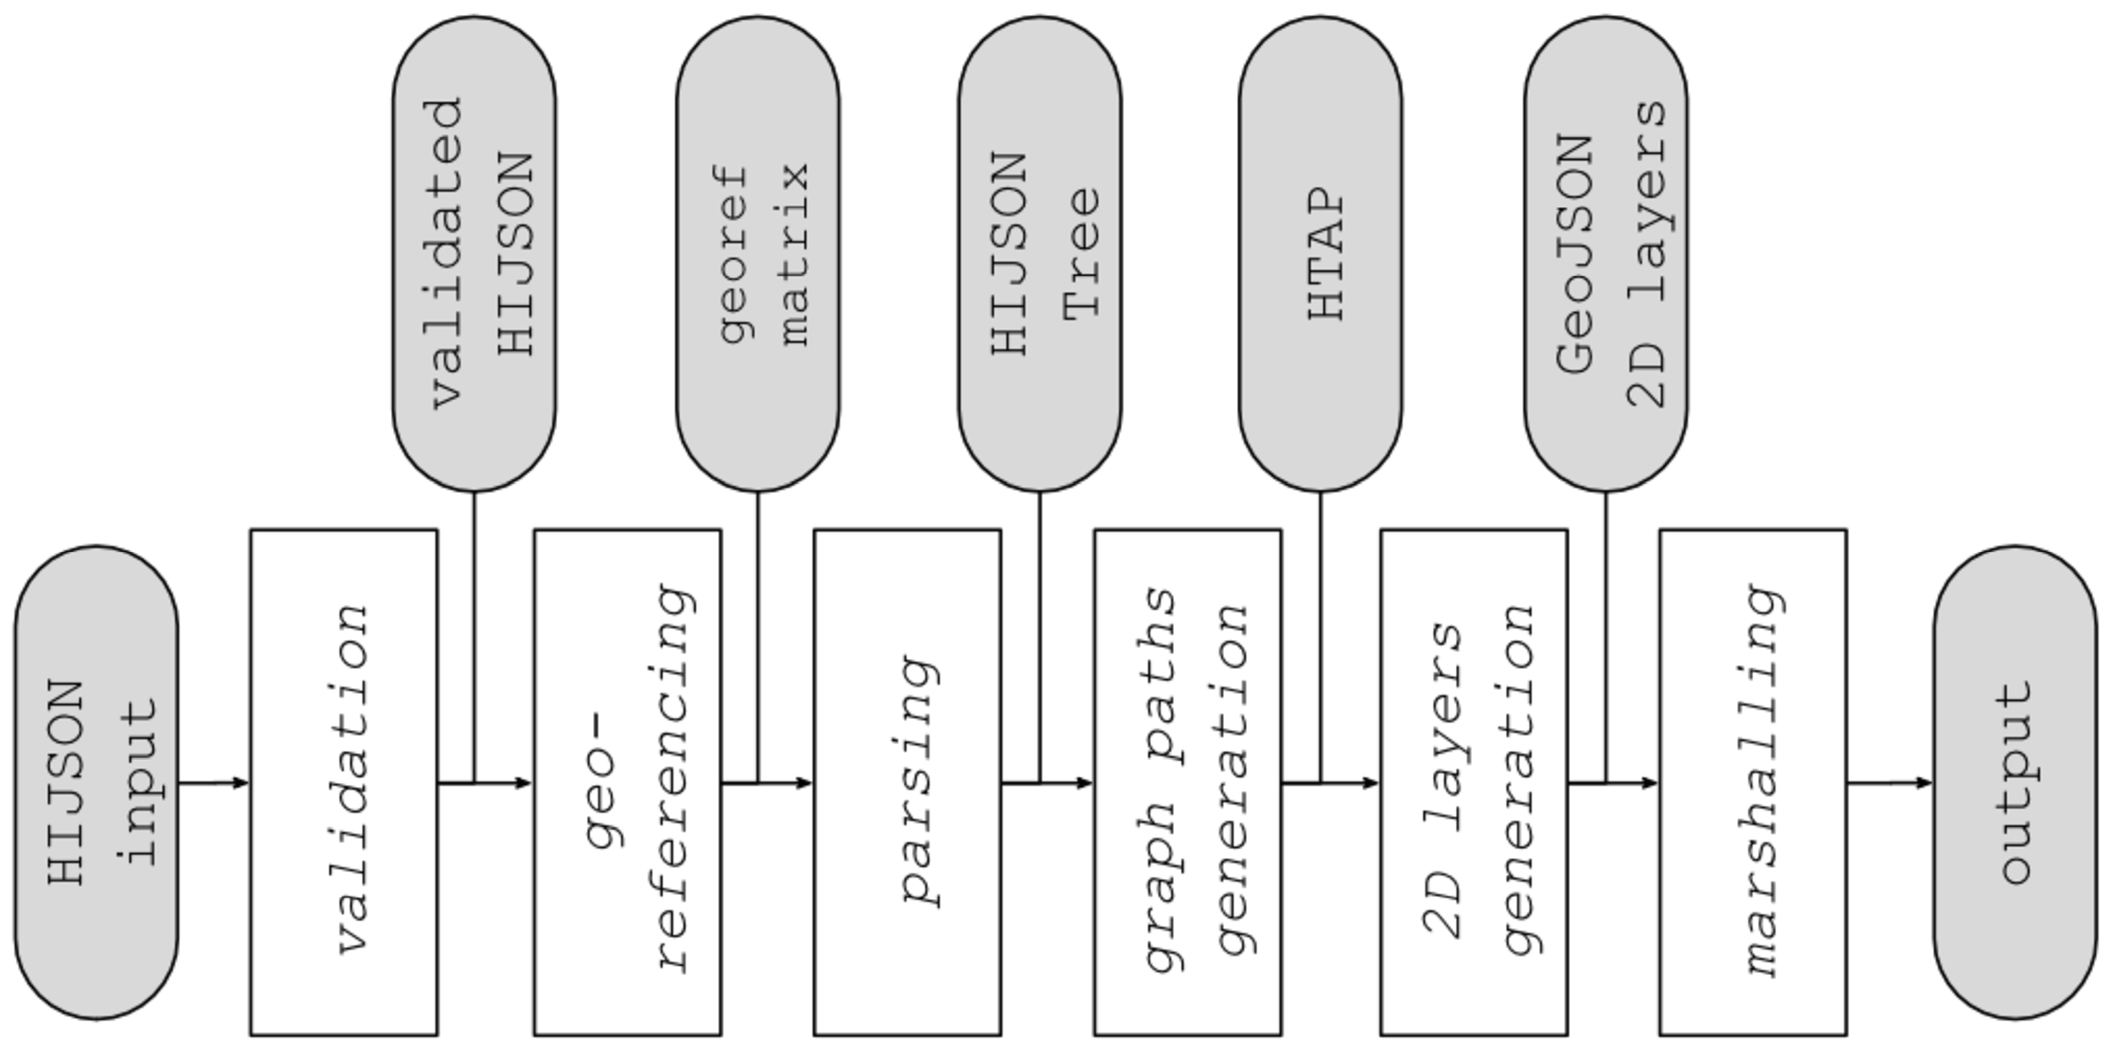
\includegraphics[width=.8\linewidth]{../images/pipeline-2}
\caption{HiJson processing pipeline}
\label{fig:pipeline}
\end{figure}

\begin{figure}[!h]
\centering
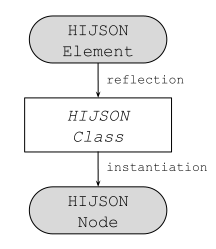
\includegraphics[width=.8\linewidth]{../images/element-class-node}
\caption{HIJSON Element/Class/Node relashionship}
\label{fig:elem-class-node-rel}
\end{figure}


\paragraph{Automatic generation of valid paths}

The graph generated, although non optimal, ensures a complete coverage of the surface while limiting the number of generated nodes. The resulting graph is weighted on the edges with nodes distances. 

The graph of paths allows for calculations of directions between any two given nodes. Although different approaches have been explored [3], a very classical solution has been selected in this case, so directions are actually computed client-side by applying the Dijkstra algorithm to the graph.

Taking advantage of the hierarchical structure of the HiJson document, and according to the divide et impera approach, the problem of paths generation is split in several sub-problems, which consist in the computation of the sub-graphs relative to each individual space, more generally a single room. 

\paragraph{HiJson Class definition}

To make better use of the possibilities offered by the HiJson Toolkit and by the HiJson document format, some custom dynamic behaviors can be described. These behaviors encapsulate the specificities relative to communication protocols with the sensors, as well as to features of user interaction. The interface for such behavior is the HiJson Class.
Every Element of the input HiJson document has a dynamic counterpart, a running instance called  Node, instantiated according to the corresponding Class via reflection methods.


User's needs for new indoor elements, greatly different sensor equipments, alternative representations of 2D or 3D viewports are accepted by the definition of new HiJson Classes, that so provide single-point custom extensions of the Toolkit capabilities.

\subsection{HiJson web framework}

The HiJson Web Framework responds to the needs of an extendable, customizable, and scalable web framework which provides at the same time IoT monitoring, realtime multi-person tracking and cross-storey user navigation.

Expandability and customizability derive from both design choices and HiJson inherent characteristics, i.e. the possibility of semantic extensions. Scalability is directly borrowed from technologies used for software development: JavaScript language, using Node.js, in particular Express.js as backend framework, exploiting the power of WebSocket protocol through the Socket.io library.

Being supported by the web-as-a-platform, the framework exposes also an high availability: it is so simple to use as to visit a website, both from desktop or mobile devices, without explicit requirements to install any software package from proprietary stores|access to which is often denied from business devices.

\paragraph{Applications}

The Framework has been designed with focus on two different kind of users: the Explorer and the Supervisor. They have different requirements and are likely equipped with different devices: while the Supervisor monitors the indoor environment through a desktop workstation, the Explorer has a smartphone available and needs to be routed across the building.

In both cases, the web platform ensures a perfect alignment with the BYOD (Bring Your Own Device) approach, nowadays often supported by companies that encourage employees to use personal devices.


\begin{figure}[htb]
\centering
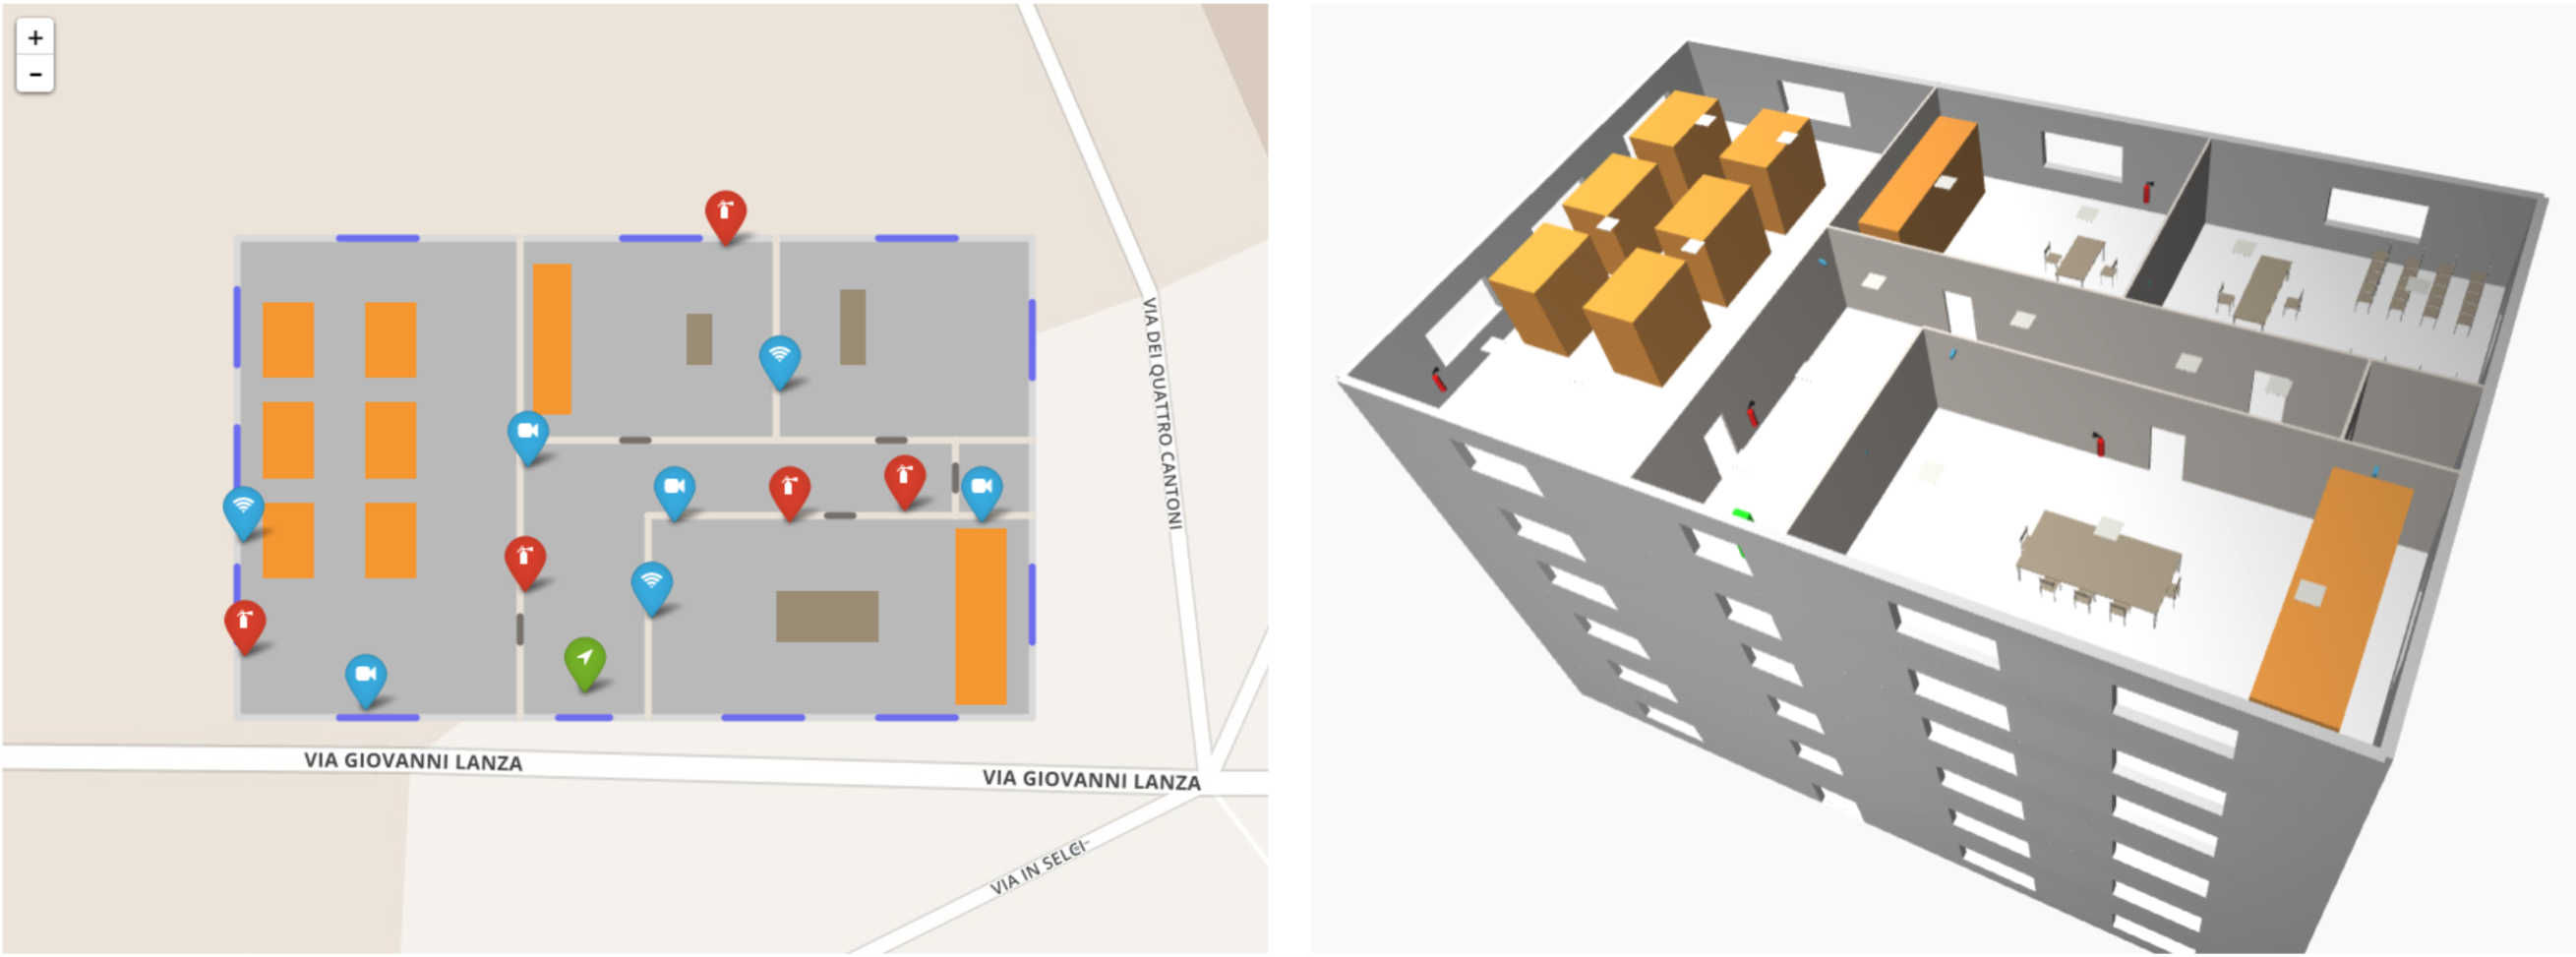
\includegraphics[width=\linewidth]{../images/2D-3D}
\caption{HiJson Web Framework UI}
\label{fig:web-framework-ui}
\end{figure}

\paragraph{IoT monitoring}

An IoT monitoring application consists of an interface showing to the user, in a single, integrated and centralized way, the information collected from all the smart objects modelled in the HiJson document. IoT monitoring application provides bidirectional communication, since the interface let the user receive information coming from smart objects while allowing him to send commands to them.

As the name itself may suggest, it is an activity specifically performed by a Supervisor user, but it can be also suitable to be deployed for the Explorer user, since she can take advantage of the interactive information coming from the surroundings objects while she moves across the indoor environment.

Monitoring different smart objects may require different ways to visualize and/or send data and commands. In particular, the user interface is characterized by a dual-display mode, that allows the user to see at the same time a 2D map that gives an overall glance in a simplified plan, and a 3D virtual environment to navigate into, as shown in Figure 6.

Alongside with typical smart objects, suitable to deal with like thermostats, where the user can read the room temperature and turn the heating on/off, other kinds of objects, that are not properly considered ``smart", can be integrated into the HiJson environment. It is the case, for example, of fire extinguishers, that are able to show the date of their last check, stored in a database.

\paragraph{Realtime multi-person tracking}
Realtime multi-person tracking allows a Supervisor to monitor the current real position of people inside the building. This kind of task can be useful for several reasons, including security, logistics or to supervise composite operative workflows. Each device equipped with the Explorer application is in charge of locating itself, interacting with the indoor positioning system, and notifying the current position in continuos mode. Evidence of the people position is given to the Supervisor both into a 2D map and an immersive 3D virtual environment (see Figure 6).

\paragraph{Cross-storey user navigation}
The HiJson Framework also provides the capability to give directions to Explorer users that must move across the indoor environment. The user specifies a starting and an ending point and the system provides him with a valid connection path. This feature strongly rely on the graph of paths generated by the Toolkit, so starting and ending points must be nodes of the graph. Connection nodes are introduced to represent stairs or elevators, enabling cross-storey paths to be computed. Since paths can span more than one storey, the most effective way to display them to the user is to show the connection nodes visualized in one or more 2D maps.


\section{Conclusions}

In this paper a novel document format, named HiJson, for indoor cartographical descriptions has been introduced. Utilization of local metric coordinate system, avoiding the manipulation of global geographical coordinates, really inconvenient when dealing with indoor spaces and objects, greatly enhances the modeling and rendering of the document content. Currently, we produce the HiJson document from a python script using two libraries for geometric computing (pyplasm and larcc [7, 14, 6]). The modeling process can be further improved by implementing a LAR-based graphical editor to assist the user during the description of the indoor space. The realization of such an editor is already in our plans.
On the basis of this representation a virtual web environment can be rebuilt working as a unifying platform to run a bunch of different applications. The reference architecture of such a platform has been also implemented and described in this work.
The architecture supports a whole range of applications: IoT monitoring, realtime multi-person tracking and user crossstorey navigation are already implemented and described. A very convenient way to extend the representation capabilities of smart objects is also mentioned as semantic extensions. These extensions, which affects both document format and its web framework, might be easily collected in a public repository. Community could both use public available extensions or contribute by mapping new (smart) objects inside the HiJson document format.

\bibliographystyle{abbrv}
\bibliography{doceng2015}  % sigproc.bib is the name of the Bibliography in this case

\end{document} 